\documentclass[12pt, letterpaper]{article}
\usepackage{bbold}
\usepackage{indentfirst}
\usepackage{amsmath, amssymb}
\usepackage[T1]{fontenc}
\usepackage[utf8]{inputenc}
\usepackage{physics}
\usepackage{tensor}
\usepackage{braket}
\usepackage{graphics}
\usepackage{grffile}
\graphicspath{ {/home/noor/Project/}}
\newcommand*{\1}{\hspace{1pt}}
\author{Noor E Mustafa Ferdous}

\title{}

\date{}

\begin{document}
    \maketitle
    
    \section*{Ans for (a)}
    
     The Partiton fucntion 

    \begin{equation}
        Z[J] = \mathcal{N}_{0} e^{V[\frac{\partial}{\partial J_{i}}]} e^{\frac{1}{2} J_{m} \Delta _{mn} J_{n}}
    \end{equation}

    Where 
    \begin{align}
        V[\phi] = \frac{\lambda}{4!} \phi = \frac{\lambda}{4!}\frac{\partial}{\partial J_{i}}
    \end{align}

    expanding the equation 

    \begin{equation}
    \begin{split}
        Z[J] = [1 + \frac{\lambda}{4!}(\frac{\partial}{\partial J_{i}})^{4} + {\frac{\lambda}{4!}}^{2}(\frac{\partial}{\partial J_{i}})^{4}(\frac{\partial}{\partial J_{i}})^{4} + .....] \mathcal{N}_{0} e^{\frac{1}{2} J_{m} \Delta _{mn} J_{n}}
    \end{split}
    \end{equation}

    Contribution of the first order in lambda
    \begin{align}
        \frac{\lambda}{4!}\frac{\partial ^4}{{\partial J_{i}}^4} [e^{\frac{1}{2} J_{m} \Delta _{mn} J_{n}}]
    \end{align}
    
    Now, taking $e^{\frac{1}{2}J_{m}\Delta_{mn}J_{n}}=U$
    \begin{align}
        \frac{\partial}{\partial J_{i}} e^{\frac{1}{2}J_{m}\Delta_{mn}J_{n}} = \Delta_{im}J_{m}U 
    \end{align}

    Again    
    \begin{equation}
    \begin{split}
        \frac{\partial^2}{{\partial J_{i}}^2} e^{\frac{1}{2}J_{m}\Delta_{mn}J_{n}} = \Delta_{ii}U + (J_{m}\Delta_{im})^{2} U
    \end{split}
    \end{equation}
    
    Again    
    \begin{equation}
    \begin{split}
        \frac{\partial^3}{{\partial J_{i}}^3} e^{\frac{1}{2}J_{m}\Delta_{mn}J_{n}} = \Delta_{ii}\Delta_{ii}U + (J_{m}\Delta_{im})^{3} U + 2J_{m}\Delta_{im}\Delta_{ii} U 
    \end{split}
    \end{equation}

    Again    
    \begin{equation}
    \begin{split}
        \frac{\partial^4}{{\partial J_{i}}^4} e^{\frac{1}{2}J_{m}\Delta_{mn}J_{n}} = 3\Delta_{ii}\Delta_{ii}U + (J_{m}\Delta_{im})^{4} U + 6(J_{m}\Delta_{im})^{2}\Delta_{ii} U 
    \end{split}
    \end{equation}

    Therefore the partiton function upto first order of lambda is
    \begin{align}
        Z[J] = [1+\frac{\lambda}{4!}3\Delta_{ii}\Delta_{ii}U + (J_{m}\Delta_{im})^{4} U + 6(J_{m}\Delta_{im})^{2}\Delta_{ii} U]\mathcal{N{_0}}
    \end{align}
    
    Second order of lambda will be
    \begin{equation}
        \frac{\lambda ^4}{(4!)^4}(\frac{\partial}{\partial J_{i}})^{4}(\frac{\partial}{\partial J_{j}})^{4}U = \frac{\lambda}{4!}[3\Delta_{ii}\Delta_{ii}U + (J_{m}\Delta_{im})^{4} U + 6(J_{m}\Delta_{im})^{2}\Delta_{ii} U]
    \end{equation}

    First term of equation 10 will be
    \begin{equation}
        \frac{\lambda ^4}{(4!)^4}(\frac{\partial}{\partial J_{j}})^{4}3\Delta_{ii}\Delta_{ii}U = 3\Delta_{ii}\Delta{ii}[3\Delta_{jj}\Delta_{jj}U + (J_{m}\Delta_{jm})^{4} U + 6(J_{m}\Delta_{jm})^{2}\Delta_{jj} U]
    \end{equation}

    Second term of equation 10 will be
    \begin{align*}
        \frac{\lambda ^4}{(4!)^4}(\frac{\partial}{\partial J_{j}})^{4}(J_{m}\Delta_{im})^{4} U &  = 6\Delta_{ii}[12\Delta_{ij}^{2}\Delta{jj}U + 12\Delta_{ij}^{2}\Delta_{jn}J_{n}\Delta_{jn}J_{n}U \\ 
        & \  + 8\Delta_{in}J_{n}\Delta_{ij}\Delta_{jj}\Delta_{jn}J_{n}U + 16\Delta_{in}J_{n}\Delta_{ij}\Delta_{jj}\Delta_{jn}J_{n}U \\ 
        & \  + 8\Delta_{in}J_{n}\Delta_{ij}(\Delta_{jn}J_{n})^{3}U + (\Delta_{in}J_{n})^{2}\Delta_{jj}(\Delta_{jn}J_{n})^{2}U + 2(\Delta_{in}J_{n})^{2}\Delta_{jj}^{2}U  \\ 
        & \  + 2(\Delta_{in}J_{n})^{2}\Delta_{jj}(\Delta_{jn}J_{n})^{2}U + 3(\Delta_{in}J_{n})^{2}\Delta_{jj}(\Delta_{jn}J_{n})^{2}U \\ 
        & \  + (\Delta_{in}J_{n})^{2}(\Delta_{jn}J_{n})^{4}U + (\Delta_{in}J_{n})^{2}\Delta_{jj}^{2}U ]
    \end{align*}
     
     Third term of the equation 10 
     \begin{align*}
        \frac{\lambda ^4}{(4!)^4}(\frac{\partial}{\partial J_{j}})^{4} &  = 24\Delta_{ij}^{4}U + 48\Delta_{in}J_{n}\Delta_{ij}^{3}\Delta_{jn}J_{n}U + 60(\Delta_{in}J_{n})^{2}\Delta_{ii}^{2}(\Delta_{jn}J_{n})^{2}U \\ 
        & \ \  + 16(\Delta_{in}J_{n})^{3}\Delta_{ij}\Delta_{jj}(\Delta_{jn}J_{n})^{2}U + 32(\Delta_{in}J_{n})^{3}\Delta_{ij}\Delta_{jj}\Delta_{jn}J_{n}U \\ 
        & \ \  + 16(\Delta_{in}J_{n})^{3}\Delta_{ij}(\Delta_{jn}J_{n})^{3}U + (\Delta_{in}J_{n})^{4}\Delta_{jj}(\Delta_{in}J_{n})^{2}U + 2(\Delta_{in}J_{n})^{4}\Delta_{jj}^{2}U \\ 
        & \ \  + 2(\Delta_{in}J_{n})^{4}\Delta_{jj}^{2}U + 2(\Delta_{in}J_{n})^{4}\Delta_{jj}(\Delta_{jn}J_{n})^{2}U + 3(\Delta_{in}J_{n})^{4}\Delta_{jj}(\Delta_{jn}J_{n})^{2}U \\ 
        & \ \  + (\Delta_{in}J_{n})^{4}\Delta_{jj}^{2}U + (\Delta_{in}J_{n})^{4}(\Delta_{jn}J_{n})^{4}U
     \end{align*}

     Therefore 
     \begin{align*}
        \frac{\lambda ^4}{(4!)^4}(\frac{\partial}{\partial J_{i}})^{4}(\frac{\partial}{\partial J_{j}})^{4}U & = 3\Delta_{ii}\Delta{ii}[3\Delta_{jj}\Delta_{jj}U + (J_{m}\Delta_{jm})^{4} U + 6(J_{m}\Delta_{jm})^{2}\Delta_{jj} U] \\
        & \  +  6\Delta_{ii}[12\Delta_{ij}^{2}\Delta{jj}U + 12\Delta_{ij}^{2}\Delta_{jn}J_{n}\Delta_{jn}J_{n}U \\ 
        & \  + 8\Delta_{in}J_{n}\Delta_{ij}\Delta_{jj}\Delta_{jn}J_{n}U + 16\Delta_{in}J_{n}\Delta_{ij}\Delta_{jj}\Delta_{jn}J_{n}U \\ 
        & \  + 8\Delta_{in}J_{n}\Delta_{ij}(\Delta_{jn}J_{n})^{3}U + (\Delta_{in}J_{n})^{2}\Delta_{jj}(\Delta_{jn}J_{n})^{2}U + 2(\Delta_{in}J_{n})^{2}\Delta_{jj}^{2}U  \\ 
        & \  + 2(\Delta_{in}J_{n})^{2}\Delta_{jj}(\Delta_{jn}J_{n})^{2}U + 3(\Delta_{in}J_{n})^{2}\Delta_{jj}(\Delta_{jn}J_{n})^{2}U \\ 
        & \  + (\Delta_{in}J_{n})^{2}(\Delta_{jn}J_{n})^{4}U + (\Delta_{in}J_{n})^{2}\Delta_{jj}^{2}U ] \\
        & \ + 24\Delta_{ij}^{4}U + 48\Delta_{in}J_{n}\Delta_{ij}^{3}\Delta_{jn}J_{n}U + 60(\Delta_{in}J_{n})^{2}\Delta_{ii}^{2}(\Delta_{jn}J_{n})^{2}U \\ 
        & \ \  + 16(\Delta_{in}J_{n})^{3}\Delta_{ij}\Delta_{jj}(\Delta_{jn}J_{n})^{2}U + 32(\Delta_{in}J_{n})^{3}\Delta_{ij}\Delta_{jj}\Delta_{jn}J_{n}U \\ 
        & \ \  + 16(\Delta_{in}J_{n})^{3}\Delta_{ij}(\Delta_{jn}J_{n})^{3}U + (\Delta_{in}J_{n})^{4}\Delta_{jj}(\Delta_{in}J_{n})^{2}U + 2(\Delta_{in}J_{n})^{4}\Delta_{jj}^{2}U \\ 
        & \ \  + 2(\Delta_{in}J_{n})^{4}\Delta_{jj}^{2}U + 2(\Delta_{in}J_{n})^{4}\Delta_{jj}(\Delta_{jn}J_{n})^{2}U + 3(\Delta_{in}J_{n})^{4}\Delta_{jj}(\Delta_{jn}J_{n})^{2}U \\ 
        & \ \  + (\Delta_{in}J_{n})^{4}\Delta_{jj}^{2}U + (\Delta_{in}J_{n})^{4}(\Delta_{jn}J_{n})^{4}U
     \end{align*}
    \section*{Ans for (b)}

    Partition up to first order of lambda 
    \begin{align}
        Z[J] = [1 + \frac{\lambda}{4!}(\frac{\partial}{\partial J_{i}})^{4}]\mathcal{N}_{0} e^{\frac{1}{2} J_{m} \Delta _{mn} J_{n}}
    \end{align}


    The two point function is
    \begin{align*}
        \langle \phi_{x}\phi_{y} \rangle & = \frac{1}{Z[0]}\frac{\partial ^2 Z[J]}{\partial J_{x} \partial J_{y}}\Biggr|_{J=0} \\
        & =  \frac{1}{Z[0]}\frac{\partial ^2 }{\partial J_{x} \partial J_{y}}  [1+\frac{\lambda}{4!}3\Delta_{ii}\Delta_{ii}U + (J_{m}\Delta_{im})^{4} U \\
        & \ \ \  + 6(J_{m}\Delta_{im})^{2}\Delta_{ii} U]\mathcal{N}_{0} e^{\frac{1}{2} J_{m} \Delta _{mn} J_{n}}\Biggr|_{J=0}
    \end{align*}

    As we are taking J=0, the  $(J_{m}\Delta_{im})^{4} U$ term will become zero.
    \begin{align*}
         &\frac{\partial ^2 Z[J]}{\partial J_{x} \partial J_{y}}  [U+\frac{\lambda}{4!}3\Delta_{ii}\Delta_{ii}U + (J_{m}\Delta_{im})^{2}\Delta_{ii} U] \\
         & = \frac{\partial }{\partial J_{y}}[\frac{\partial}{\partial J_{x}} + U \frac{\lambda}{4!}(3\Delta_{ii}\Delta_{ii}\Delta_{xm}J_{m} + 12\Delta_{xi}J_{m}U\Delta_{im}\Delta_{ii})] \\ 
         & = [\Delta_{xy} + \frac{\lambda}{4!}(3\Delta_{ii}\Delta_{ii}\Delta_{xy} + 12\Delta_{xi}\Delta_{ii}\Delta_{iy})]
    \end{align*}

    Therefore the two point function
    \begin{align}
        \langle \phi_{x}\phi_{y} \rangle & = \frac{\Delta_{xy} + \frac{\lambda}{4!}(3\Delta_{ii}\Delta_{ii}\Delta_{xy} + 12\Delta_{xi}\Delta_{ii}\Delta_{iy})}{1+\frac{\lambda}{4!} 3\Delta_{ii}\Delta_{ii}}
    \end{align}

    Binomial expanding the lower part of the fraction we get
     \begin{align}
        \langle \phi_{x}\phi_{y} \rangle & = [\Delta_{xy} + \frac{\lambda}{4!}( 3\Delta_{ii}\Delta_{ii}\Delta_{xy} + 12\Delta_{ix}\Delta_{ii}\Delta_{iy})][1-\frac{\lambda}{4!} 3\Delta_{ii}\Delta_{ii}] \\
        & = \Delta_{xy} + \frac{\lambda}{4!}(12\Delta_{ix}\Delta_{ii}\Delta_{iy})
    \end{align}

    \section*{Ans for (c)}

    So the diagram will be 
    \begin{figure}[h]
    \centering
    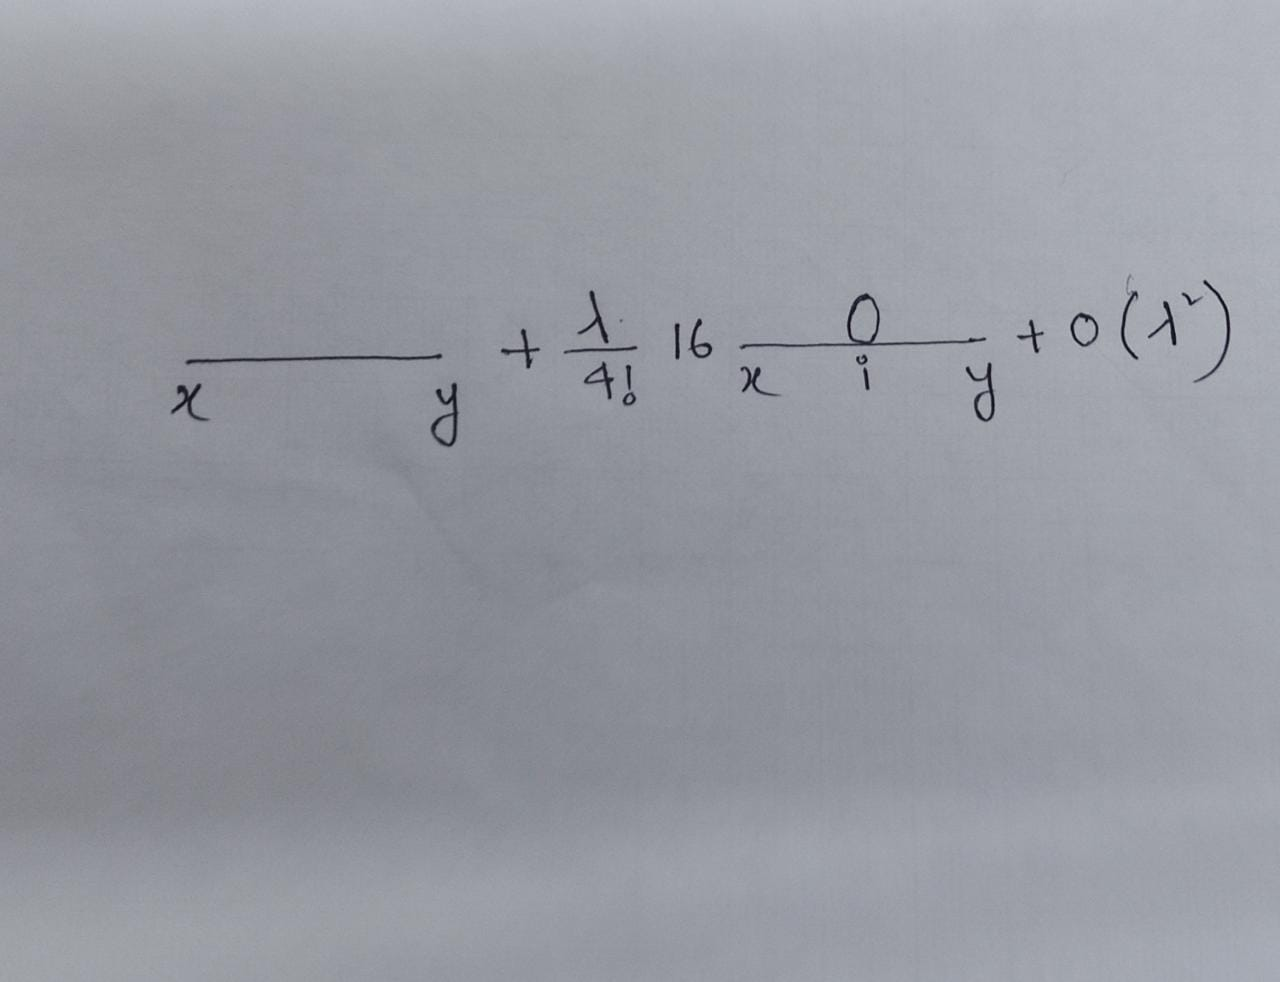
\includegraphics[scale=.05]{pic}
    \end{figure}

\end{document}